\chapter{Power and Sample Size \label{chapter:powersamplesize}}

%%%%%%%%%%%%%%%%%%%%%%%%%%%%%%%%%%%%%%%%%%%%%%%%%%%%%%%%%%%%%%%%%%%%%%%%%%%%%%%%

\section{Statistical Power}

\textbf{Power} is the probability that a hypothesis test will reject the null hypothesis if the alternative hypothesis is, in fact, true. The graph below shows two distributions: the sampling distribution under the null (mean $\mu_0$) and the sampling distribution under the alternative hypothesis (mean $\mu_1$). Note that these sampling distributions are for the \emph{test statistic}; it could be the sample mean, sample proportion, sample correlation coefficient, sample difference in means, etc.

\begin{center}
%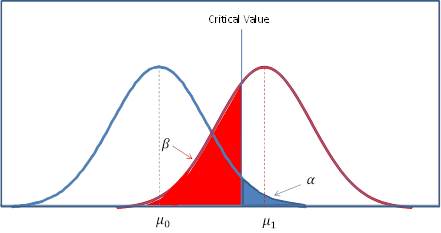
\includegraphics[width=0.65\textwidth]{img/statistical-power-chart.png}
\end{center}

\begin{mdframed}
\textbf{Question 2.8:} There are three ways to increase the power of a hypothesis test. (Hint: Have a look at the parameters in the formula for the $T$-test statistic, above.) Try to list them here:
\begin{enumerate}
\item ~
\item ~
\item ~
\end{enumerate}
\vspace{5mm}
\end{mdframed}

%%%%%%%%%%%%%%%%%%%%%%%%%%%%%%%%%%%%%%%%%%%%%%%%%%%%%%%%%%%%%%%%%%%%%%%%%%%%%%%%

\section{Sample Size Calculations}

For many statistical hypothesis tests, we can reverse the calculation and ask: how many samples do we need at a certain effect size to reject the null at a given significance level? Even in cases where you can't invert the test statistic itself, you can often use \textbf{bootstrapping}, \textbf{permutations}, etc. to simulate the appearance of the data under the null. 

This graph shows the number of samples required to detect the effect size shown in the Appalachian town example in the slides ($\overline{x} = 125.45$, $\mu_0 = 139.75$) at varying significance levels: $\alpha = 0.1$ (orange line), $\alpha = 0.05$ (blue dotted line), and $\alpha = 0.01$ (turquoise dashed line). 

\begin{center}
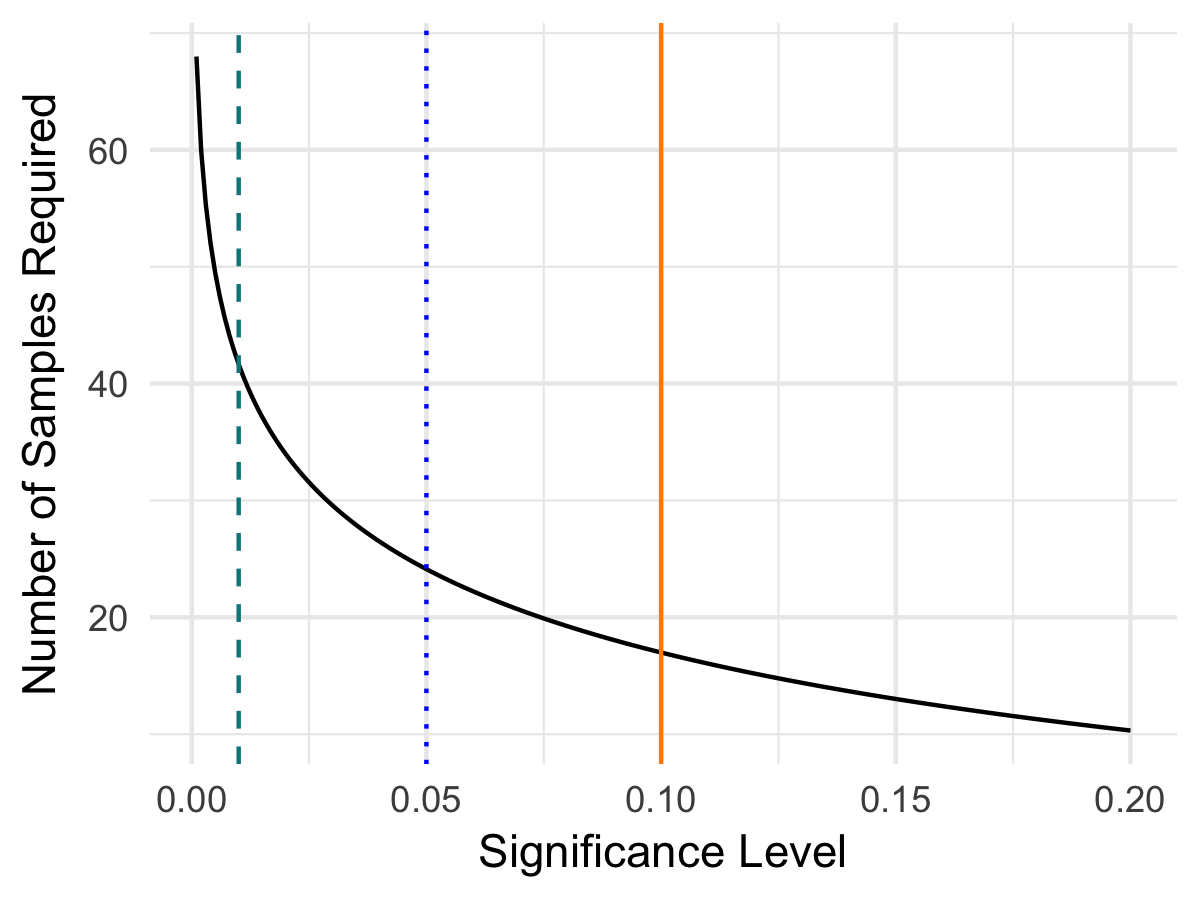
\includegraphics[width=0.5\textwidth]{img/hyp-z-test-power-curve-1.png}
\end{center}

Now let's vary the effect size. The graph below shows three lines, representing the sample sizes needed to reject the null at $\alpha = 0.1$ (solid), $0.05$ (dotted), and $0.01$ (dashed) significance levels, using a two-sided test.

\begin{center}
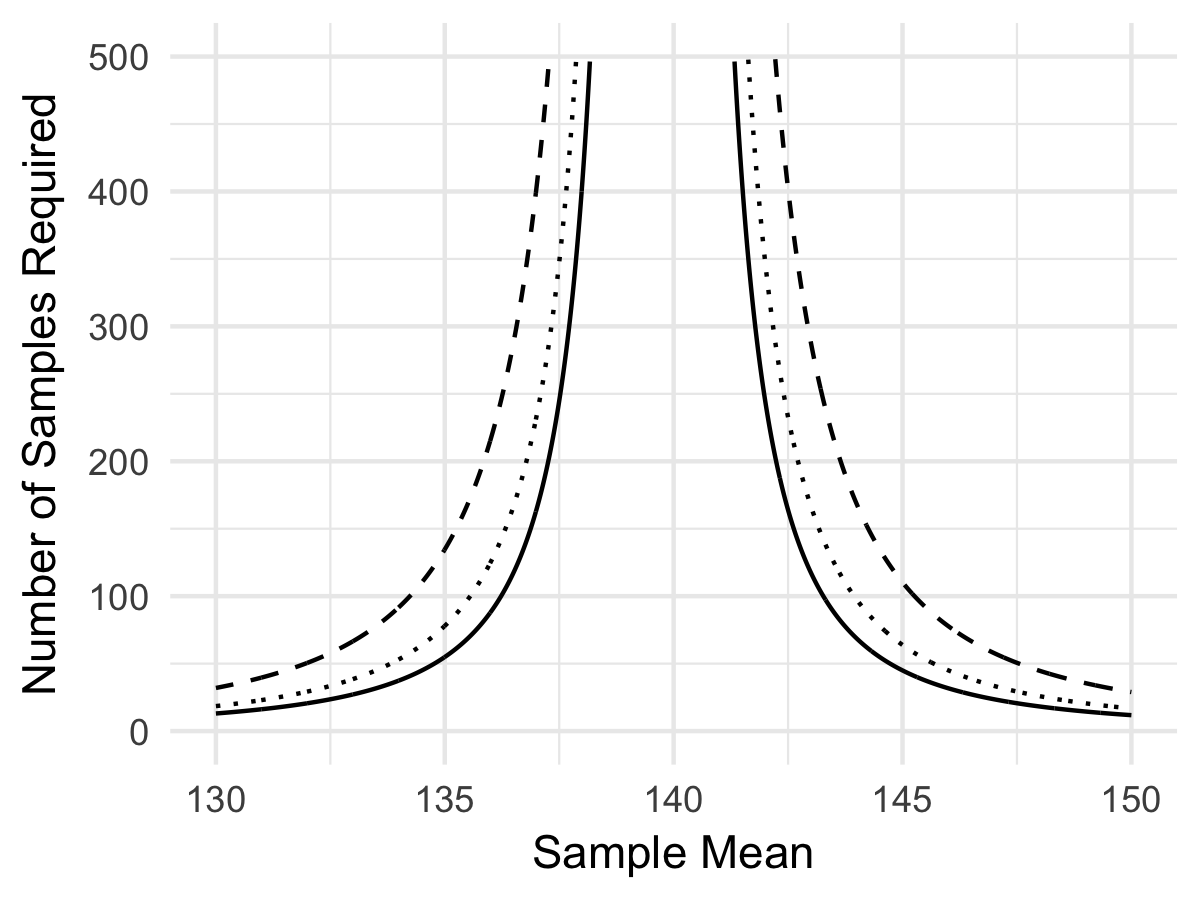
\includegraphics[width=0.5\textwidth]{img/hyp-z-test-power-curve-2.png}
\end{center}
